\documentclass{article}

% set font encoding for PDFLaTeX or XeLaTeX
\usepackage{ifxetex}
\ifxetex
  \usepackage{fontspec}
\else
  \usepackage[T1]{fontenc}
  \usepackage[utf8]{inputenc}
  \usepackage{lmodern}
  \usepackage{graphicx}
  \usepackage{float}

\fi

% used in maketitle
\title{Tiro parabólico Con Resistencia Al Aire}
\author{Eduardo Hndz\\Universidad De Sonora\\Lic. En Física}

% Enable SageTeX to run SageMath code right inside this LaTeX file.
% documentation: http://mirrors.ctan.org/macros/latex/contrib/sagetex/sagetexpackage.pdf
% \usepackage{sagetex}

\begin{document}
\maketitle

\section {Tiro Parabólico}
En esta actividad nos tocó realizar un programa para calcular la velocidad y posición de un proyectil el cual se enfrente a la resistencia del aire.
para ellos utilizamos el metodo de euler ya que la ecución es de tipo diferencial y no contabamos con los conocimientos de dicha materia.
\subsection {Código}
El código que realicé es el siguiente, tiene varios comentarios ya que tuve errores de tipo lógico y prefiero no volver a cometerlos en un futuro.
\begin{verbatim}
 program prueba_arrastre
  implicit none
  !declaramos constantes!
  !debemos poner contador para cada Do
  !utilizaremos un mismo ángulo pero velocidades variadas
  integer::k,l,i,Vo
  integer,parameter:: ntimes=1000
  real,parameter:: Pi=3.1415927 , g=9.8 , delt=0.01, theta=45*Pi/180
  real,parameter:: m=0.142, cd=0.47, ro=1.225, r=0.035
  real::A, Vt,C,t,Voa
  !Declaramos variables,utilizamos arreglos de vectores (cajitas de vectores)
  real,dimension(1:ntimes):: X,Y,Vx,Vy
!calculamos el área del cuerpo a estudiar
  A=Pi*(r*r)
  Vt=sqrt((2*m*g)/(ro*A*cd))
  print*, Vt
!calculamos el coeficiente de arrastre de dicho cuerpo
  C=(m*g)/(Vt)
  Print*, C
!comenzamos con un contador, el cual va a variar la velocidad inicial
  !de nuestro objeto a estudiar, comenzando en 10 hasta 100 en
  !intervalos de 10
 open(1,file='datosarrastre.dat', status='unknown')
  do Vo=10,100,10
    Voa=float(Vo)
  !comenzar un ciclo para las primeras dos posiciones, donde se
    !infiere que no hay resistancia al aire
    !recuerda siempre revisar las ecuaciones y apuntes, porque te
    !salía mal por eso
    !recuerda poner el cualquier variable que  vayas a usar dentro
    !del loop, dentro de este, no que te salía mal por eso -.-
    do i=1,2
        t=float(i)*delt
     Vx(i)=Voa*cos(theta)
     Vy(i)=Voa*sin(theta)-g*t
     X(i)=Vx(i)*t
     Y(i)=Vy(i)*t-(0.5*g*(t*t))
 
     print*,  Vx(i), Vy(i) , X(i), Y(i)
    write(1,*) X(i), Y(i)
  end do
  
  !ahora calcularemos donde la particula ya se opone al aire
  !dado que ya tenemos los primeros dos datos, comenzaremos a
  !calcular aparte de la tercera posición de dicha particula
  do  i=3,ntimes
 
     t=float(i)*delt
     Vx(i)=Vx(i-1)-((Vx(i-1)*delt*C/m))
     X(i)=x(i-1)+((delt)*Vx(i-2))-((delt)*(delt)*Vx(l)*c/m)
     Vy(i)=Vy(i-1)*(1-delt*C/m)-delt*g
     Y(i)=Y(i-1)+(delt*Vy(i-2)-(delt*delt*Vy(i-2)*C/m)-delt*delt*g)

     if(Y(i)<0) exit
     write(1,*) X(i), Y(i)
     
  end do
  end do
  !siempre que tu loop es el más externo, se cierra hasta el final.
 close(1)
 end program prueba_arrastre


\end{verbatim}
El resultado de mi programa fue el siguiente.
\begin{figure}[h!]
  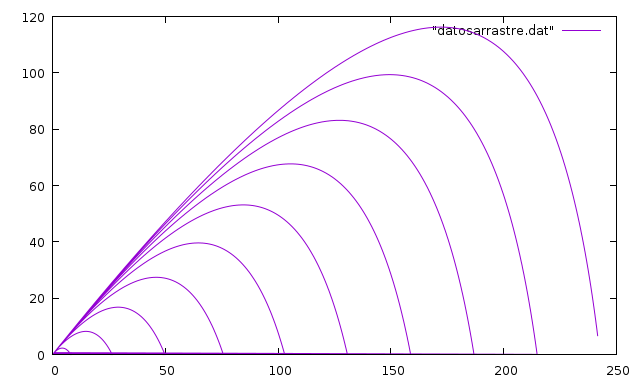
\includegraphics[width=\linewidth]{arraste.png}
  \caption{final}
  \label{fig:boat1}
\end{figure}
\end{document}
